% Words Before Tokens? Locating lexical information in byte-level Indic-script LMs.
% Compile: tectonic paper.tex   (or: latexmk -pdf paper.tex)
% Switch to anonymous review mode: change \usepackage[final]{acl} to \usepackage[review]{acl}
\documentclass[11pt]{article}
\PassOptionsToPackage{hidelinks}{hyperref}
\usepackage[final]{acl}
\usepackage{times}
\usepackage{latexsym}
\usepackage[T1]{fontenc}
\usepackage[utf8]{inputenc}
\usepackage{microtype}
\usepackage{graphicx}
\usepackage{booktabs}
\usepackage{amsmath}
\usepackage{amssymb}
\usepackage{multirow}
\usepackage{xcolor}

\newcommand{\x}{$\times$}

\title{Words Before Tokens? Locating a Word's Information in\\
Byte-Level Indic-Script Language Models}

\author{Rochit L. \\
  \texttt{rochitl72@gmail.com} \\
  \texttt{github.com/rochitl72/research-paper}}

\begin{document}
\maketitle

\begin{abstract}
Byte-level BPE tokenizers split a Tamil or Hindi word into five to ten
tokens, while an English word is usually one. We ask where, inside such a
fragmented word, the model's information about \emph{which} word it is
actually lives, and whether that information can be read, moved, or exploited.
Measuring per-token surprisal on Qwen3-0.6B and 1.7B over Tamil, Hindi and
English Wikipedia, we find that the first token of an Indic word carries
almost none of the word's information---$8\%$ for Tamil and $27\%$ for Hindi,
against $96\%$ for English---because nearly every word begins with the same
shared script bytes; a second model family whose tokenizer fragments Indic far
less puts the information back in the first token, showing the effect is
tokenizer-driven, not a property of the script. A linear probe on the hidden
state \emph{before} the word
is written identifies the upcoming word far above dictionary and control
baselines, and stays ahead of the written prefix as the word unfolds. Yet this
information is not a localized ``plan'': activation patching of the pre-word
position transfers the donor word in under $8\%$ of matched natural-context
pairs, while a first-token-position control reaches $100\%$; attention
knockout nonetheless shows the pre-word position is a \emph{necessary relay},
costing about two bits and halving correct spelling when blocked. Every finding
replicates across two model sizes and a second model family. Guided by this
picture, we build a lossless word-level speculative decoder from linear heads
that fit in under two minutes on a laptop; it produces token-for-token
identical greedy output at $1.5$--$2.0$ tokens per forward pass and up to
\x$1.9$ wall-clock speedup on an M1 GPU, with gains that grow with model size.
Code, data pipeline and all results are released.
\end{abstract}

\section{Introduction}

A language model that writes Tamil or Hindi does far more sequential work per
word than one writing English. Under the byte-level BPE tokenizer shared by
most modern models \citep{radford2019gpt2,sennrich2016bpe}, a Tamil word is
split into $9.6$ tokens on average and a Hindi word into $4.8$, against $1.1$
for English. Each of those tokens is one sequential forward pass at
generation time, so the same sentence costs several times more latency and
money in an Indic script than in English---a disparity documented for
tokenization cost and fairness \citep{petrov2023tokenizers,ahia2023costs}.

This paper starts from a simple question about the \emph{internal} side of that
disparity. When a model is partway through spelling out a long Indic word, how
much of its decision about \emph{which} word this is has already been made, and
\emph{where} in the computation does that decision live? A natural hypothesis,
which we call \emph{words before tokens}, is that the model commits to a whole
word at the position just before it starts writing it, and the remaining tokens
are near-deterministic spelling. If true, this would be both scientifically
interesting---a word-level plan under a sub-word interface---and practically
useful: the spelling tokens could be drafted in parallel and verified in one
pass, recovering the latency lost to fragmentation, with no change to the
output distribution.

We test this hypothesis directly on Qwen3-0.6B-Base and Qwen3-1.7B-Base
\citep{qwen2024} over Tamil, Hindi and English Wikipedia, and find that it is
half right in an informative way.

\begin{itemize}
\item \textbf{The first token says almost nothing} (\S\ref{sec:spelling}).
  Because nearly every Tamil word begins with the same token---a space plus the
  UTF-8 lead bytes shared across the script---only $8\%$ of a Tamil word's
  information (in bits) sits in its first token, versus $96\%$ for English.
  The information is spread across the interior tokens and never falls to zero.
\item \textbf{The word is readable before it is written} (\S\ref{sec:probe}).
  A linear probe on the pre-word hidden state picks the upcoming word out of
  1{,}000 candidates well above a most-frequent-word baseline and a
  control-task baseline \citep{hewitt2019control}, and is far more accurate on
  words the model goes on to spell correctly. As the word unfolds, the state
  stays $10$--$27$ points ahead of what the written prefix alone reveals.
\item \textbf{But the word is not localized or decided there}
  (\S\ref{sec:causal}). Activation patching \citep{meng2022rome,wang2023ioi} of
  the pre-word position moves the next-token decision at most a tenth of the way
  toward a donor word, while patching the first in-word position reaches $100\%$
  at the last layer. Attention knockout shows the other half: the pre-word
  position is a \emph{necessary} relay---blocking it costs about two bits and
  halves correct spelling---whose content nonetheless does not carry the choice
  of word. The word is re-derived from the whole context at each step.
\item \textbf{A lossless decoder exploits what is there}
  (\S\ref{sec:decoder}). We train cheap linear ``word heads'' and Medusa-style
  token-ahead heads \citep{cai2024medusa,gloeckle2024multitoken} on frozen
  features and use them as drafters in a draft-then-verify loop whose output is
  provably identical to greedy decoding. On a MacBook M1 Pro the best drafter
  reaches $2.0$ tokens per forward pass on Tamil and up to \x$1.9$ wall-clock on
  Hindi, and the speedup grows from the $0.6$B to the $1.7$B model.
\end{itemize}

Every result is reported for both model sizes; the qualitative picture is
identical across scale and the quantitative effects sharpen with it. Our
contribution is primarily a measurement and a mechanism---\emph{where} lexical
information lives under byte-level tokenization and how it is (and is not)
organized---together with a working, laptop-reproducible lossless decoder that
puts the mechanism to use. We release the full code, the data pipeline, and
the raw results that generate every number and figure here.

\section{Related Work}

\paragraph{Tokenization and language cost.} Byte-level BPE
\citep{sennrich2016bpe,radford2019gpt2} guarantees that any string can be
encoded, but allocates its vocabulary budget toward the training mix, so
scripts under-represented in that mix fragment into many tokens.
\citet{petrov2023tokenizers} and \citet{ahia2023costs} quantify the resulting
unfairness in sequence length, context usage and API cost across languages.
We take this fragmentation as given and ask what it does to the model's
\emph{internal} representation of a word, and whether the extra tokens are
cheap to predict.

\paragraph{Speculative and parallel decoding.} Speculative decoding
\citep{leviathan2023speculative,chen2023speculative} accelerates generation by
drafting tokens with a cheap proposer and verifying them in one pass of the
target model, leaving the output distribution unchanged. Blockwise parallel
decoding \citep{stern2018blockwise}, Medusa \citep{cai2024medusa} and EAGLE
\citep{li2024eagle} replace the separate draft model with extra heads on the
target model itself, and multi-token prediction \citep{gloeckle2024multitoken}
trains such heads from scratch. Our decoder is in this family, with two
differences of emphasis: the draft unit is a whole \emph{word} (a span the
tokenizer fragmented), and the heads are fit by convex optimization on frozen
features so the whole thing runs on a laptop. Closest in motivation,
\citet{yi2024multilingual} speed up multilingual inference with
language-specific \emph{draft models}; we instead target the within-word
fragmentation directly, with per-language word heads on the target model's own
features and no separate draft model. We use these methods as a lens on the
representation question rather than to chase state-of-the-art throughput.

\paragraph{Probing and causal analysis.} Linear probes
\citep{alain2017probes} measure what is linearly decodable from a hidden
state; control tasks \citep{hewitt2019control} guard against probes that
succeed by memorization rather than by reading structure, and we adopt their
shuffled-label control throughout. To ask whether decodable information is
\emph{causal} we use the logit-lens / tuned-lens view of the residual stream
\citep{belrose2023tunedlens,elhage2021framework} and activation patching
\citep{meng2022rome,wang2023ioi,goldowskydill2023pathpatching}, patching
between two natural contexts rather than synthetic edits. The combination of a
positive probe, a negative patching result and a positive knockout result is
what lets us separate ``readable'' from ``stored here'' from ``needed here''.

\paragraph{Reading and planning future tokens.} Closest to our probe, Future
Lens \citep{pal2023futurelens} shows that several upcoming tokens can be
anticipated from a single hidden state. \citet{wu2024planahead} ask whether
this reflects deliberate \emph{pre-caching} of future-token features or mere
\emph{breadcrumbs} left by computation useful for the present token, and find
natural language modeling is mostly breadcrumbs at small scale. We make both
questions concrete for a unit the tokenizer has shattered: whether the identity
of a whole multi-token \emph{word} is decodable before it is written in a
heavily fragmented script, and---unlike these works---we pair the probe with
patching and knockout to test whether that information is a localized stored
plan (pre-caching) or re-derived from context at each step (breadcrumbs). For
Indic words the answer is the latter, with the pre-word position acting only as
a necessary relay.

\section{Setup and definitions}
\label{sec:setup}

\paragraph{Models.} We study Qwen3-0.6B-Base and Qwen3-1.7B-Base
\citep{qwen2024}: same tokenizer and depth (28 transformer blocks), hidden
size $1024$ and $2048$ respectively. Both are base (non-instruct) models, run
in float32 on a MacBook M1 Pro (16\,GB, Metal/MPS). All analysis is
teacher-forced: we never sample, so every number is deterministic given the
text.

\paragraph{Data.} For each language we take 6{,}000 consecutive paragraphs from
the \texttt{wikimedia/wikipedia} 20231101 dumps, filtered to $80$--$600$
characters. Paragraphs $0$--$3999$ form a ``fit'' pool (for training probes and
heads) and $4000$--$5999$ a held-out ``eval'' pool; experiments use the first
$1{,}500$ fit and $500$ eval paragraphs, truncated to $256$ tokens. Splitting
by paragraph range, not at random, keeps whole articles on one side of the
split.

\paragraph{Words and boundaries.} We segment each token sequence into
\emph{units} by decoding the bytes of each token and marking a new word unit at
a token that begins with a space (or a script word break). A \emph{word} unit
with $n>1$ tokens has one \emph{first token} and $n-1$ \emph{continuation
tokens}. For each continuation token we label the boundary it opens as:
\textbf{byte}, if it falls inside a single UTF-8 character; \textbf{grapheme},
if it falls inside one written syllable (a Unicode grapheme cluster); or
\textbf{subword}, a split between whole graphemes. Byte- and grapheme-internal
splits are artifacts of the encoding; only subword splits are linguistic.

\paragraph{Definitions.} For a continuation token with model probability $p$
under teacher forcing, we call it \emph{near-certain} at threshold $\tau$ if
$p \ge \tau$. The \emph{spelling share} at $\tau$ is the fraction of all word
tokens that are near-certain continuations---the share of generation steps a
perfect drafter could skip. We measure a word's information as its total
surprisal in bits, $-\log_2 p$ summed over its tokens, and report the
\emph{first-token share}: the fraction of a word's bits contributed by its
first token, averaged over words. A low first-token share means the first token
is predictable (shared across the vocabulary) and the word's identity is
decided later.

\section{The first token of an Indic word carries almost no information}
\label{sec:spelling}

\begin{table}[t]
\centering\small
\begin{tabular}{lrrr}
\toprule
 & Tamil & Hindi & English \\
\midrule
Tokens / word & 9.59 & 4.82 & 1.14 \\
Multi-token words & 96.4\% & 98.9\% & 9.3\% \\
\midrule
\multicolumn{4}{l}{\emph{Spelling share} (word tokens near-certain at $p\ge\tau$)}\\
\quad $\tau=0.5$ & 46.4 / 53.5 & 43.7 / 50.1 & 7.5 / 8.5 \\
\quad $\tau=0.9$ & 27.6 / 35.1 & 28.5 / 35.9 & 5.2 / 6.3 \\
\quad $\tau=0.99$ & 12.4 / 19.0 & 14.2 / 21.1 & 2.6 / 3.7 \\
\midrule
First-token share & 7.7 / 8.2 & 24.9 / 26.7 & 94.7 / 95.8 \\
\bottomrule
\end{tabular}
\caption{Where a word's information lives. Cells with two numbers are
Qwen3-0.6B / Qwen3-1.7B. The first token holds almost none of a Tamil or Hindi
word's information; confidence in continuation tokens rises with model size.}
\label{tab:spelling}
\end{table}

Table~\ref{tab:spelling} reports the core measurement. Three things stand out,
and all three hold for both model sizes.

\textbf{Indic words fragment, and the first token is shared.} A Tamil word is
$9.6$ tokens and a Hindi word $4.8$, versus $1.1$ for English; $96\%$ of Tamil
and $99\%$ of Hindi words are multi-token, against $9\%$ of English words. The
first-token share is only $8\%$ for Tamil and $25$--$27\%$ for Hindi, but
$95$--$96\%$ for English. The reason is mechanical: nearly every Tamil word
begins with the same token---a leading space followed by the UTF-8 lead bytes
common to the whole Tamil Unicode block---so that token is almost free to
predict and the word's identity must be resolved by the tokens that follow.
This is the precise internal counterpart of the fragmentation cost of
\citet{petrov2023tokenizers}: not only are there more tokens, the \emph{first}
one is nearly contentless.

\textbf{Where the bits are.} Figure~\ref{fig:bits} plots mean surprisal by
token position within a word. For Tamil the information is concentrated in the
second and third tokens and then settles a little above one bit per token for
the rest of the word---it never reaches zero, so most ``spelling'' tokens still
carry a residual decision. This already bounds any decoder: the continuation is
not free.

\textbf{Encoding vs.\ linguistic boundaries.} Of Tamil continuation tokens,
$36\%$ open a byte-internal boundary and $27\%$ a grapheme-internal one; only
$37\%$ are splits between whole graphemes. The encoding-internal splits are the
\emph{more} predictable ones ($40\%$ near-certain at $\tau=0.9$ for byte splits
vs.\ $17\%$ for grapheme splits on $0.6$B), because completing a half-written
character is often forced. A decoder that skips tokens therefore gets its
easiest wins on splits that are artifacts of UTF-8, not on linguistic
structure.

\begin{figure}[t]
\centering
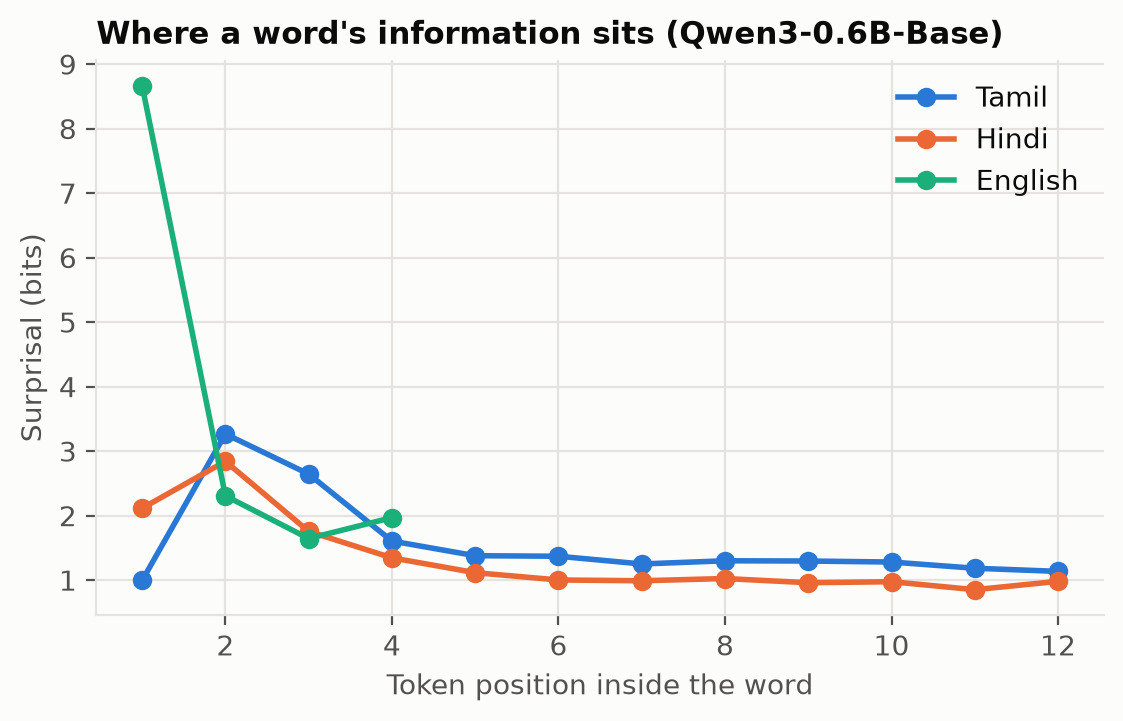
\includegraphics[width=\columnwidth]{../figures/Qwen3-0.6B-Base/fig2_bits_by_position.png}
\caption{Mean surprisal (bits) by token position within a word, Qwen3-0.6B.
The information of a Tamil/Hindi word is concentrated in its first few interior
tokens and then plateaus above zero; an English word is decided at token one.}
\label{fig:bits}
\end{figure}

The spelling share at $\tau=0.9$---the fraction of steps a perfectly confident
drafter could skip---is $27.6\%$ for Tamil on $0.6$B and rises to $35.1\%$ on
$1.7$B. We set $40\%$ as an a-priori bar for ``most of the word is spelling'';
neither model clears it, but the gap narrows with scale and $63$--$69\%$ of
continuation tokens are already greedy-correct, which is what the decoder in
\S\ref{sec:decoder} actually exploits.

\paragraph{A second family confirms the tokenizer is the cause.} To check that
this is a property of the \emph{tokenizer} and not of the languages, we repeat
the measurement on XGLM-564M \citep{xglm2022}, a different family whose
SentencePiece tokenizer was trained with heavy multilingual (including Indic)
coverage. It fragments Indic words far less, and the first-token share rises in
lockstep (Table~\ref{tab:family}): a Tamil word is $2.5$ tokens instead of
$9.6$, and $57\%$ of its information is now in the first token instead of $8\%$.
The phenomenon tracks fragmentation, not script: a model whose tokenizer spends
vocabulary on Indic behaves, for Tamil and Hindi, much more like it does for
English. The low first-token share under byte-level BPE is therefore a cost of
the tokenizer, and the internal correlate of the sequence-length unfairness of
\citet{petrov2023tokenizers}.

\begin{table}[t]
\centering\small
\begin{tabular}{lrrrr}
\toprule
 & \multicolumn{2}{c}{Tokens / word} & \multicolumn{2}{c}{First-token share} \\
 & Qwen3 & XGLM & Qwen3 & XGLM \\
\midrule
Tamil   & 9.59 & 2.54 & 7.7\%  & 56.5\% \\
Hindi   & 4.82 & 1.46 & 24.9\% & 81.6\% \\
English & 1.14 & 1.21 & 94.7\% & 92.8\% \\
\bottomrule
\end{tabular}
\caption{Cross-family check (Qwen3-0.6B byte-level BPE vs XGLM-564M
SentencePiece). The less a tokenizer fragments a word, the more of the word's
information sits in its first token. The effect is tokenizer-driven, not
language-intrinsic.}
\label{tab:family}
\end{table}

\section{The word is readable before it is written}
\label{sec:probe}

If the word's information is not in the first token, is it anywhere by the time
the model is about to write the word? We train a linear probe on the pre-word
hidden state---the state at the last context token, before any of the word is
emitted---to predict the upcoming word among the $1{,}000$ most frequent
multi-token words. Because byte-level BPE gives almost all Tamil words the same
first token, we cannot restrict candidates by first token as one would in
English; we predict the whole word identity. We compare against two baselines:
the most-frequent-word rate (dictionary prior) and a shuffled-label control
task \citep{hewitt2019control}. We also split test accuracy by whether the
model itself goes on to spell the word correctly.

\begin{table}[t]
\centering\small
\begin{tabular}{lrrrr}
\toprule
Layer & Probe & Most-freq. & Control & Chance \\
\midrule
\multicolumn{5}{l}{\emph{Tamil} (1000 classes, 4{,}515 held-out)}\\
\quad 7  & 12.7 / 13.6 & 3.2 & 1.5 & 1.0 \\
\quad 14 & 13.6 / 15.3 & 3.2 & 1.5 & 1.0 \\
\quad 21 & 14.5 / 16.6 & 3.2 & 1.5 & 1.0 \\
\quad 28 & 14.2 / 16.4 & 3.2 & 1.7 & 1.0 \\
\midrule
\multicolumn{5}{l}{\emph{Hindi} (1000 classes, 16{,}370 held-out)}\\
\quad 7  & 34.8 / 35.4 & 24.4 & 14.1 & 1.2 \\
\quad 14 & 36.3 / 38.1 & 24.4 & 14.5 & 1.2 \\
\quad 21 & 39.5 / 42.6 & 24.4 & 14.8 & 1.2 \\
\quad 28 & 39.8 / 43.5 & 24.4 & 15.3 & 1.2 \\
\bottomrule
\end{tabular}
\caption{Pre-word plan probe (\% accuracy, $0.6$B / $1.7$B where two numbers).
The probe beats both the dictionary prior and the shuffled-label control at
every layer, and readability sharpens with model size.}
\label{tab:probe}
\end{table}

Table~\ref{tab:probe} shows the probe beats both baselines at every layer and
for both models. Tamil reaches $14.5\%$ ($0.6$B) and $16.6\%$ ($1.7$B) against
a $3.2\%$ dictionary prior and a $1.5\%$ control; Hindi reaches $39.8$/$43.5\%$
against $24.4\%$ and $15.3\%$. Readability rises through roughly the first
quarter of the network and then plateaus. Crucially, on words the model later
spells correctly the probe is far more accurate---$34.6\%$ vs.\ $12.0\%$ on
misspelled words for Tamil $0.6$B, $69.2\%$ vs.\ $17.8\%$ for Hindi---so the
decodable signal tracks the model's own success, not just corpus frequency.
Every probe$-$control gap is large relative to seed variation (3 seeds): Tamil
$+12.5$ points at $43$ SD and Hindi $+24.7$ at $58$ SD on $0.6$B, rising to $46$
and $83$ SD on $1.7$B.

\paragraph{As the word unfolds.} We then probe the state available after
$j=1,\dots,6$ tokens of the word have been written, against only those
candidate words consistent with the $j$-token prefix, and compare to a
prefix-only dictionary that guesses the most frequent completion of that
prefix. Table~\ref{tab:position} reports the gap. The model's state stays well
ahead of the written prefix throughout the word: for Hindi the advantage peaks
at $+23$ points ($0.6$B) / $+27$ points ($1.7$B) after two tokens, and closes
only as the prefix itself becomes unambiguous near the word's end. The model
``knows'' more about the word than it has committed to paper.

\begin{table}[t]
\centering\small
\begin{tabular}{lrrr}
\toprule
Tokens written & State & Prefix-only & Gap \\
\midrule
\multicolumn{4}{l}{\emph{Tamil} ($1.7$B)}\\
\quad 1 & 17.3 & 4.0 & +13.2 \\
\quad 2 & 32.0 & 14.7 & +17.4 \\
\quad 3 & 53.1 & 34.2 & +18.9 \\
\quad 4 & 63.0 & 48.5 & +14.5 \\
\midrule
\multicolumn{4}{l}{\emph{Hindi} ($1.7$B)}\\
\quad 1 & 43.6 & 24.5 & +19.1 \\
\quad 2 & 67.9 & 41.2 & +26.7 \\
\quad 3 & 80.0 & 61.3 & +18.6 \\
\quad 4 & 85.5 & 75.1 & +10.5 \\
\bottomrule
\end{tabular}
\caption{Word identity as the word unfolds (\% accuracy, Qwen3-1.7B). The
hidden state identifies the word earlier than its written prefix does.}
\label{tab:position}
\end{table}

\section{The word is necessary but not localized at the pre-word position}
\label{sec:causal}

A probe shows a feature is \emph{present} and linearly decodable, not that the
model \emph{uses} it or that it is \emph{stored} where the probe reads. We run
two causal tests, both on natural text, to decide this.

\paragraph{Activation patching.} We mine pairs of real contexts $(A,B)$ in
which the model confidently and greedily writes two different multi-token words
$X$ and $Y$ that share their first token. We then run context $B$ while
overwriting the residual stream at $B$'s pre-word position, at one layer, with
$A$'s activation from the same position, and measure how far the next-token
logit difference moves toward $X$ (``effect'', normalized so $1.0$ = fully
A-like), and whether the model then spells $X$ out in full (``transfer''). As a
control we patch the first \emph{in-word} position instead.

The pre-word patch is weak at every layer and every scale: the median effect
peaks around $0.08$ (Tamil) and $0.18$ (Hindi) in the middle layers and decays
to zero by the last, and the donor word is spelled out in at most $4$--$6\%$ of
pairs. The first-token-position control, by contrast, grows monotonically to an
effect of $1.00$ at the last layer and transfers the full donor word in up to
$44\%$ (Tamil) / $38\%$ (Hindi) of pairs (Figure~\ref{fig:patching}). In other
words, the choice of word is \emph{not} sitting at the pre-word position waiting
to be executed; it is assembled over the course of the word, and the position
that accumulates the causal signal is the one \emph{inside} the word, late in
the network. This directly contradicts the ``words before tokens'' hypothesis
in its strong form. The contrast is unambiguous: at the last layer the
first-token control transfers the donor word in $21$--$44\%$ of pairs while the
pre-word patch transfers it in none, with no pair showing the reverse (McNemar
$p<10^{-4}$ for every model and language).

\begin{figure}[t]
\centering
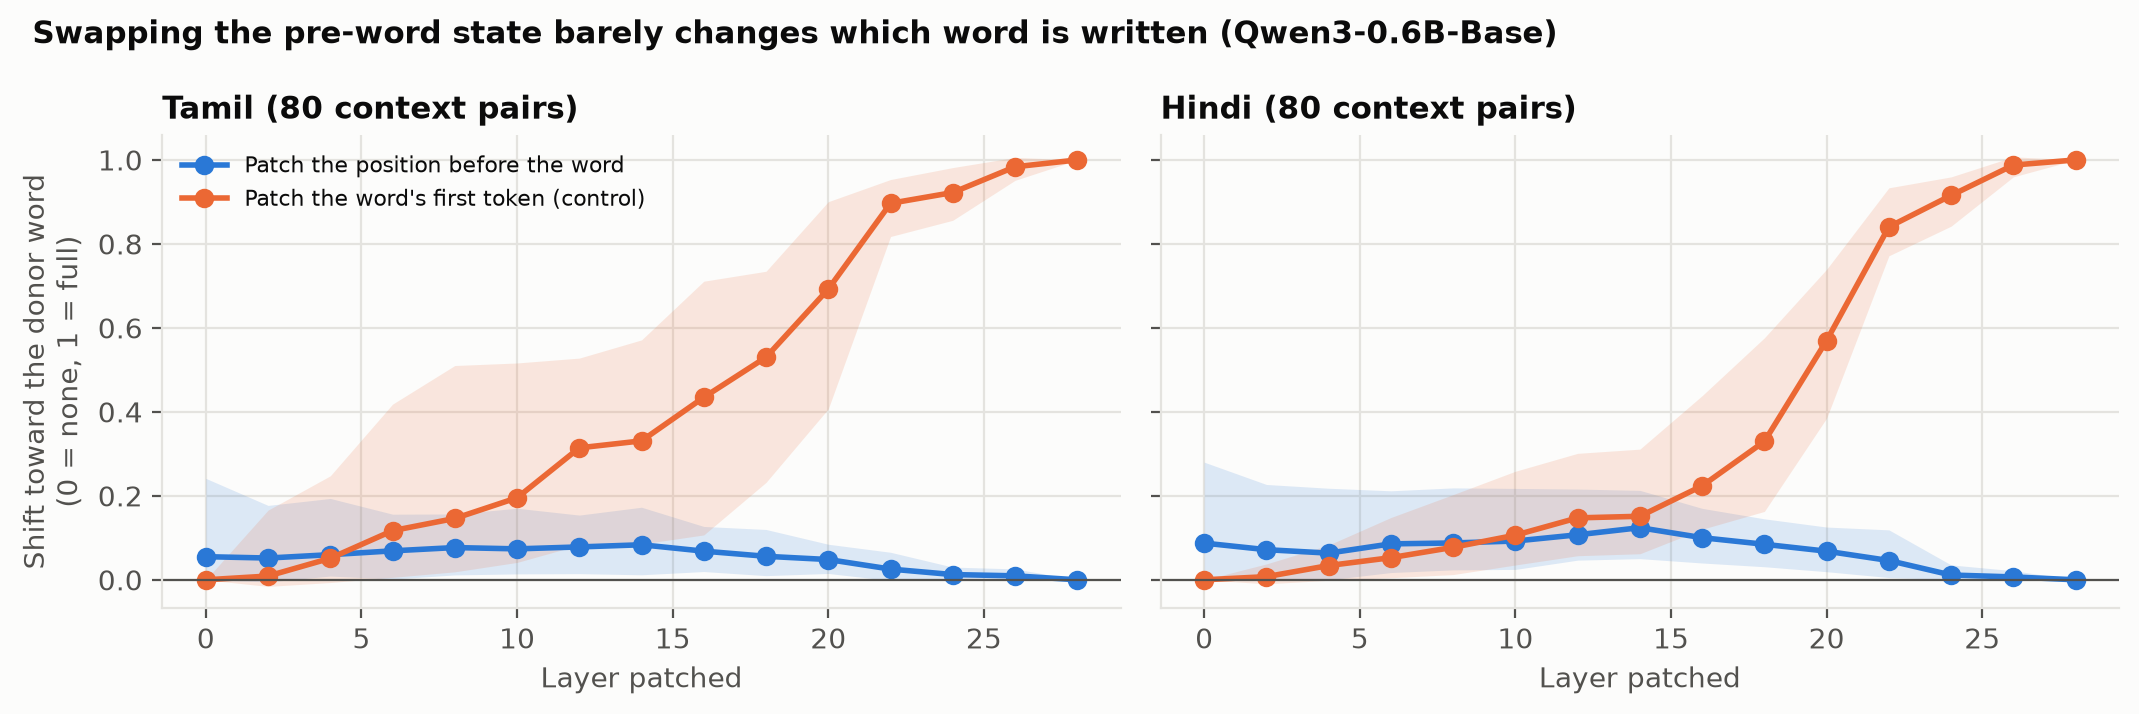
\includegraphics[width=\columnwidth]{../figures/Qwen3-0.6B-Base/fig5_patching.png}
\caption{Activation patching, Qwen3-0.6B. Swapping the pre-word state (blue)
barely changes which word is written; swapping the first in-word position
(orange control) takes over the decision by the last layer. The word is not
localized before it is written.}
\label{fig:patching}
\end{figure}

\paragraph{Attention knockout.} Patching asks whether the pre-word content
\emph{determines} the word; knockout asks whether it is \emph{needed} at all.
For words the model spells correctly, we block attention from the word's own
positions to one earlier position---at every layer, via an explicit additive
mask---and measure the change in the continuation's log-probability.
Table~\ref{tab:knockout} shows a sharp, local effect: blocking the pre-word
position costs $2.3$--$2.5$ bits on Tamil and $1.8$--$1.9$ on Hindi, and drops
correct spelling to $25$--$28\%$ (Tamil) and $52$--$54\%$ (Hindi). Blocking the
token just before it, or a random earlier context token, costs essentially
nothing ($\le 0.25$ bits) and leaves spelling almost intact. The pre-word cost
dwarfs the random-position control on a paired test (Wilcoxon $p<10^{-30}$ for
both languages and models); the bootstrap $95\%$ CI on the mean cost is, e.g.,
$[-2.82,-2.23]$ bits for Tamil on $1.7$B versus $[-0.05,+0.01]$ for a random
position. The result is stable across three random resamplings of the test
words: the pre-word cost is $2.3\pm0.1$ bits (Tamil) and $1.9\pm0.1$ (Hindi) on
$0.6$B, and $2.4\pm0.3$ and $1.9\pm0.1$ on $1.7$B, while the random-position
cost stays within noise of zero in every seed.

\begin{table}[t]
\centering\small
\begin{tabular}{llrr}
\toprule
Lang. & Blocked position & $\Delta$bits & Spelled \\
\midrule
Tamil & pre-word & $-2.5$ & 25\% \\
Tamil & token before that & $-0.25$ & 59\% \\
Tamil & random earlier & $-0.02$ & 61\% \\
Hindi & pre-word & $-1.9$ & 54\% \\
Hindi & token before that & $-0.03$ & 82\% \\
Hindi & random earlier & $-0.01$ & 81\% \\
\bottomrule
\end{tabular}
\caption{Attention knockout, Qwen3-1.7B (300 correctly-spelled words each).
The pre-word position is a necessary, local relay; its neighbours are not.}
\label{tab:knockout}
\end{table}

\paragraph{Reading.} The two results are complementary, not contradictory. The
pre-word position is a \emph{necessary relay}---the word's own tokens attend
back to it and lose about two bits of certainty when that link is cut---yet its
content does not \emph{carry} the identity of the word, since replacing it with
the content from a different word's context does not redirect the output. The
most consistent interpretation is that the pre-word position passes forward
local, boundary-level information (where the word starts, immediate context)
that the spelling needs, while the word's identity is recomputed from the whole
context at each interior step. This is why a probe can read the word there (the
information is linearly present in the shared context representation) even
though patching cannot move it (it is not a localized variable). It also
predicts the ceiling we hit next: a drafter that reads one early state cannot
be certain of a word that the model itself has not yet fixed.

\paragraph{The mechanism replicates on a second family.} Run on XGLM-564M, the
same picture holds and is if anything sharper: patching the pre-word position
transfers the donor word in $0\%$ of pairs for both languages while the
first-token control reaches $74\%$ (Tamil) and $89\%$ (Hindi), and knockout of
the pre-word position costs $1.4$ bits of continuation certainty against
$\le 0.06$ for a random position. The probe likewise beats its baselines
(Tamil $59\%$ vs.\ a $38\%$ control and $43\%$ dictionary prior). ``Readable,
necessary, but not localized'' is therefore not an artifact of one tokenizer or
one model family.

\section{A lossless word-level speculative decoder}
\label{sec:decoder}

The mechanism says a word is partly-but-not-fully determined in advance. We now
ask how much latency that buys back, under the hard constraint that the output
must not change at all.

\paragraph{Decoder.} At each step we take the target model's own greedy token
$t$. If $t$ begins a new word, we ask a drafter for the remaining tokens of that
word given the current hidden state; we then run a single forward pass on
$[t] + \text{draft}$ and accept drafted tokens for as long as they equal the
model's own greedy argmax, cropping the KV cache on the first rejection. Because
acceptance is defined by the target model's argmax, the output is
token-for-token identical to plain greedy decoding by construction; we also
verify this empirically on every prompt.

\paragraph{Drafters.} All drafters read frozen features and are fit by convex
optimization on the fit split, in under two minutes each on the laptop.
A \emph{word head} is a multinomial logistic regression over a lexicon
(plus an OTHER class) from a standardized hidden state; we train one on the
pre-word state and one on the current in-word state (\S\ref{sec:causal}
motivates reading the freshest state). A \emph{dictionary} drafter is the
context-blind baseline: the most frequent lexicon word consistent with the
written prefix. \emph{Token-ahead heads} are $K$ linear heads
\`a la Medusa/multi-token prediction \citep{cai2024medusa,gloeckle2024multitoken}
that predict the next $K$ tokens from the current state and token embedding over
a small output vocabulary; they need no lexicon, so they are not capped by
lexicon coverage (only $39\%$ of held-out Tamil word occurrences on the head
lexicon). We also chain them: use the word head where it has a candidate, fall
back to token-ahead heads otherwise.

\begin{table}[t]
\centering\small
\begin{tabular}{lrrrr}
\toprule
 & \multicolumn{2}{c}{Tamil} & \multicolumn{2}{c}{Hindi} \\
Drafter & tok/fwd & wall & tok/fwd & wall \\
\midrule
plain greedy & 1.00 & \x1.00 & 1.00 & \x1.00 \\
dictionary & 1.50 & \x1.43 & 1.47 & \x1.74 \\
pre-word head & 1.64 & \x1.49 & 1.70 & \x1.92 \\
current head & 1.71 & \x1.56 & 1.70 & \x1.86 \\
token-ahead heads & 1.85 & \x1.73 & 1.60 & \x1.75 \\
word + ahead & \textbf{2.00} & \x1.67 & \textbf{1.75} & \x1.83 \\
\bottomrule
\end{tabular}
\caption{Real lossless greedy decoding on Qwen3-1.7B (12 held-out prompts,
$64$ new tokens each). Output was identical to plain greedy on every prompt.
``tok/fwd'' is accepted tokens per forward pass; ``wall'' is wall-clock speedup
on the M1 GPU.}
\label{tab:decode}
\end{table}

\paragraph{Results.} Table~\ref{tab:decode} reports real decoding on the
$1.7$B model; output was identical to plain greedy on all prompts, and the same
held for $0.6$B. The best drafter reaches $2.0$ accepted tokens per forward pass
on Tamil and gives a wall-clock speedup of \x$1.67$--\x$1.73$ on Tamil and
\x$1.83$--\x$1.92$ on Hindi, even though every drafter runs in pure Python on
top of the model. Reading the model's \emph{current} state beats the
context-blind dictionary consistently, and the gain over plain decoding is
larger on $1.7$B than on $0.6$B (e.g.\ Tamil word+ahead, \x1.46 to \x1.67
wall-clock), because the fixed cost of the linear heads is amortized against a
more expensive base forward pass---the method pays off more as the model grows.
Bootstrap $95\%$ CIs over prompts put the best drafter's tokens per forward pass
clearly above one on every model and language (e.g.\ Tamil $[1.88,2.20]$ on
$1.7$B); the wall-clock speedup is noisier on throttled MPS but positive on
$9$--$11$ of $12$ prompts.
The emulated upper bound (a drafter that is always right) is \x$2.5$ fewer
passes on Tamil, so a meaningful gap remains; two things limit us, both
predicted by the mechanism: lexicon coverage is low under heavy inflection, and
the word is not fixed early (\S\ref{sec:causal}), so an early draft is often
wrong and only partially accepted. Token-ahead heads, which re-read the state
every step and need no lexicon, are the single best stand-alone drafter on
Tamil for exactly this reason.

\paragraph{The gain is proportional to fragmentation.} Running the same lossless
decoder on XGLM-564M, whose tokenizer barely fragments Indic, the best drafter
reaches only $1.1$ tokens per forward pass and no wall-clock win (Tamil
\x$1.20$, Hindi \x$0.97$)---there is almost no within-word structure left to
draft. This is the point: the method recovers latency exactly where the
tokenizer destroys it (Qwen3 Tamil, \x$1.67$) and does nothing where
tokenization is already efficient. The decoder is a remedy for fragmentation,
and its benefit scales with how badly a model's tokenizer fragments the script.

\section{Discussion and limitations}

\paragraph{What the picture is.} Byte-level tokenization does not just make
Indic words longer; it moves their information out of the first token and
spreads it across encoding-internal continuation tokens, most of which still
carry a residual decision. The upcoming word is linearly readable from the
model's state before and during writing, and that readability tracks the
model's own accuracy, but the word is not a localized variable that is set once
and executed---it is re-derived from context at each step, with the pre-word
position acting as a necessary relay rather than a store. A lossless decoder
built on this reads the freshest state, drafts a whole word, and recovers a
good part of the latency lost to fragmentation.

\paragraph{Limitations.} (i) Three models---two Qwen3 sizes and a second family,
XGLM-564M---across which every finding replicates; still, two families with
$\le 1.7$B parameters is a narrow sweep, and larger models and more families
(Gemma, Llama) are future work. (ii) Greedy decoding only; lossless
speculative \emph{sampling} needs the standard accept/reject rule, which we have
not implemented. (iii) Wall-clock numbers are batch-size-1 on Metal/MPS and
include Python-side drafter overhead; on CPU the extra draft tokens are not free
and the same decoder is slower than plain decoding. (iv) Patching uses
$50$--$80$ context pairs and knockout $300$ words; we report bootstrap $95\%$
CIs and paired tests, and seed-robustness over the random selection, but the
knockout is a whole-layer attention block, not a per-head path patch, so
``necessary relay'' is a coarse claim pending finer analysis. (v) Wikipedia text only; the 20231101 dump may overlap the models'
training data, which would inflate predictability. (vi) The causal reading in
\S\ref{sec:causal} is an interpretation consistent with three experiments, not
a validated circuit.

\section{Conclusion}

We asked where a word's information lives when a tokenizer has shattered it into
many pieces. In byte-level Indic-script models the answer is: almost nowhere in
the first token, linearly readable but not localized before the word is written,
and re-derived from context as the word unfolds. The practical consequence is a
lossless word-level speculative decoder that fits on a laptop and returns up to
twice the tokens per forward pass. We release the code, data pipeline, and the
raw results behind every figure and table so that both the measurements and the
decoder can be reproduced and extended to other scripts and model families.

\section*{Reproducibility}

All code (segmentation, corpus pass, probes, patching, knockout, heads, and the
lossless decoder), the data-building scripts, unit tests, and the raw JSON
results that generate every number and figure in this paper are available at
\url{https://github.com/rochitl72/research-paper}. Every table is produced from
\texttt{results/} by a report script; no number here is typed by hand. The full
pipeline runs on a single MacBook M1 Pro.

\bibliography{references}

\end{document}
